% !TEX TS-program = xelatex
% !TEX encoding = UTF-8
% !Mode:: "TeX:UTF-8"

\documentclass[onecolumn,oneside]{SUSTechHomework}

\usepackage{blindtext}
\usepackage{graphicx}
\usepackage{subfigure}
\usepackage{float}
\usepackage{listings}
\usepackage{hyperref}
\usepackage{framed}
\usepackage{extarrows}
\usepackage{algorithm}
\usepackage{algorithmic}
\usepackage{color}
\hypersetup{hidelinks,
	colorlinks=true,
	allcolors=black,
	pdfstartview=Fit,
	breaklinks=true}

\begin{document}

% title 
% =====================================================================
\title{Lab 7\&8: Digital Filter Design}
\sid{11812214}
\coursecode{EE323}
\coursename{Digital Signal Processing}
\author{任振裕}
\date{December 18, 2020}
\maketitle  
% Contents
\tableofcontents
% introduction
% =====================================================================
\section*{Introduction}
\addcontentsline{toc}{section}{Introduction}
This lab merges the content of Lab 7 and lab 8, which is mainly composed of two parts:
\begin{itemize}
    \item In the \textbf{first part}, we will cover some basic examples of FIR and IIR filters, and then introduces the concepts
    of FIR filter design. 
    \item In the \textbf{second part}, we will mainly discuss some systematic methods of designing FIR filters.
	\item To understand the designs of FIR and IIR digital designs, we should keep different situations of below equations in our minds all 
	the time:
	\begin{info}
		\begin{itemize}
			\item Difference equation of LTI causal digital filter (with input $x[n]$ and output $y[n]$):
			$$
			y[n]=\sum_{i=0}^{N-1} b_{i} x[n-i]-\sum_{k=1}^{M-1} a_{k} y[n-k]
			$$
			\item Impulse response, z-transform, and z-transform:
			$$
			h[n]=\sum_{i=0}^{N-1} b_{i} \delta[n-i]-\sum_{k=1}^{M-1} a_{k} h[n-k]
			$$
			$$
			H(z) \triangleq \frac{Y(z)}{X(z)}=\frac{\sum_{i=0}^{N-1} b_{i} z^{-i}}{1+\sum_{k=1}^{M-1} a_{k} z^{-k}}
			$$
			$$
			H\left(e^{j \omega}\right)=\left.H(z)\right|_{z=e^{j\omega}}=\frac{\sum_{i=0}^{N-1} b_{i} e^{-j \omega i}}{1+\sum_{k=1}^{M-1} a_{k} e^{-j \omega k}}
			$$
		\end{itemize}
	\end{info}
	\begin{info}
		\begin{itemize}
			\item For FIR filters:
			\begin{itemize}
				\item No poles, only zeros. $\rightarrow$ $a_k=0,\forall k\in \left\{1,2,...,M-1\right\}$:
				$$
				h[n]=\sum_{i=0}^{N-1} b_{i} \delta[n-i]
				$$
				\item Frequency response:
				$$
				H\left(e^{j \omega}\right)=\sum_{i=0}^{N-1} b_{i} e^{-j \omega i}
				$$
			\end{itemize}
			\item For IIR filters: Both poles and zeros exist, therefore impulse and frequency responses follow the above general forms.
		\end{itemize}
	\end{info} 
\end{itemize}
\section*{7.3 Design of a Simple FIR Filter}
\addcontentsline{toc}{section}{7.3 Design of a Simple FIR Filter}
\subsection*{Question 1:}
\begin{itemize}
	\item Analytical transfer function:
	$$
	\begin{aligned}
	H_{f}(z)&=\left(1-z_{1} z^{-1}\right)\left(1-z_{2} z^{-1}\right)
	\\&=\left(1-e^{j \theta} z^{-1}\right)\left(1-e^{-j \theta} z^{-1}\right)
	\\&=1-2 \cos \theta z^{-1}+z^{-2}
	\end{aligned}
	$$
	\item Difference equation:
	$$
	y[n]=x[n]-2 \cos \theta x[n-1]+x[n-2]
	$$
	\item The system diagram:
	\begin{figure}[H]
		\centering
		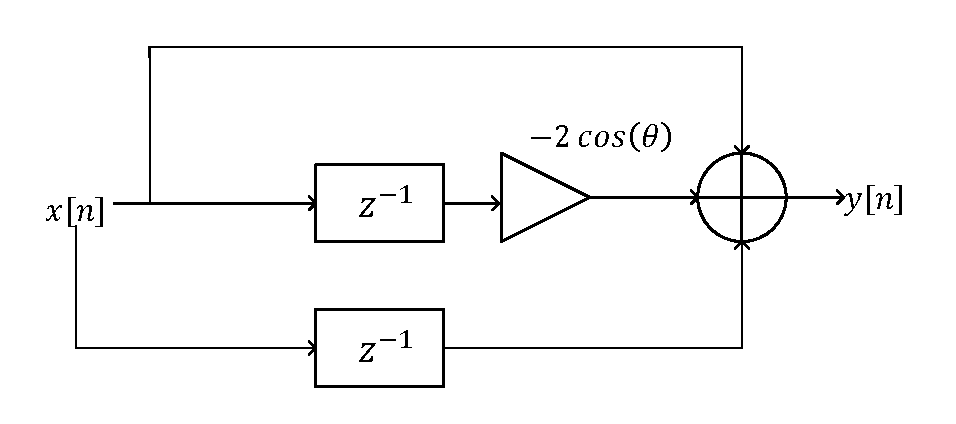
\includegraphics[width=150mm]{pictures/框图1.pdf}
		\caption{System diagram}
	\end{figure}
	\item MATLAB codes for this section:
\end{itemize}
\begin{lstlisting}[title=q7\_3a.m]
	clear;
	w = -pi:0.01:pi; z = exp(1j*w);
	H1 = 1-2*cos(pi/6)*z.^(-1)+z.^(-2);
	H2 = 1-2*cos(pi/3)*z.^(-1)+z.^(-2);
	H3 = 1-2*cos(pi/2)*z.^(-1)+z.^(-2);
	subplot(1,3,1);plot(w,abs(H1));title('\theta=\pi/6');
	subplot(1,3,2);plot(w,abs(H2));title('\theta=\pi/3');
	subplot(1,3,3);plot(w,abs(H3));title('\theta=\pi/2');
\end{lstlisting}
\begin{itemize}
	\item Running result:
	\begin{figure}[H]
		\centering
		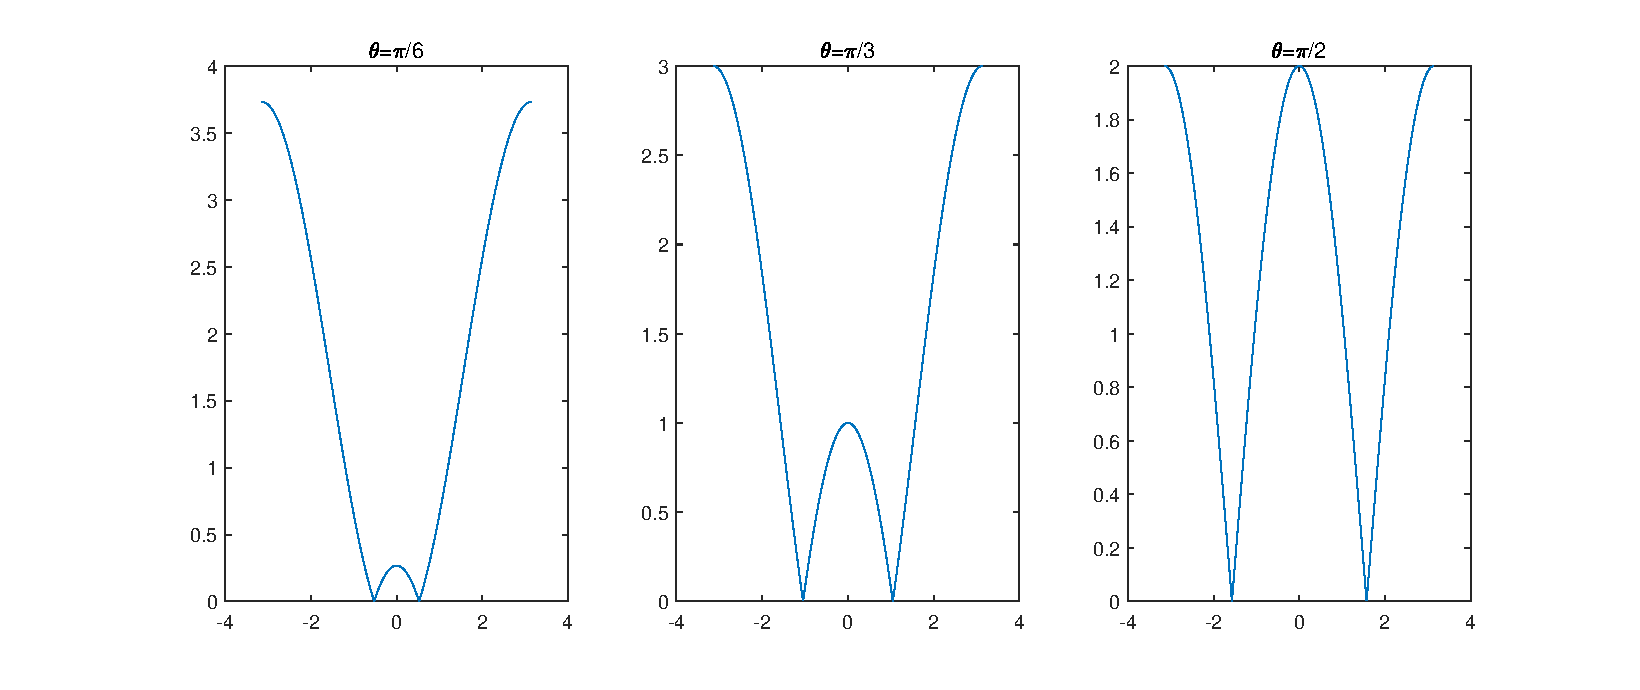
\includegraphics[width=170mm]{pictures/Hf.eps}
		\caption{$Hf$ with different $\theta$}
	\end{figure}
	\item Analysis: $\omega=\theta \rightarrow |H_f(e^{j\omega})|==0$.
\end{itemize}
\subsection*{Question 2:}
\begin{itemize}
	\item FIRfilter.m:
\end{itemize}
\begin{lstlisting}[title=FIRfilter.m]
	function y = FIRfilter(x)
	[X,w]=DTFT(x,0);
	[Xmax,Imax]=max(abs(X));
	h = [1 -2*cos(w(Imax)) 1];
	y = conv(x,h);
	end
\end{lstlisting}
\begin{itemize}
	\item q7\_3b.m:
\end{itemize}
\begin{lstlisting}[title=q7\_3b.m]
	clear;
	load nspeech1;
	y0 = FIRfilter(nspeech1);
	y1 = nspeech1(100:200);
	y2 = nspeech1(100:1100);
	y3 = y0(100:200);
	y4 = y0(100:1100);
	[X2,w2] = DTFT(y2,0);
	[Xmax,Imax] = max(abs(X2));
	[X4,w4] = DTFT(y4,0);
	subplot(221),plot([0:length(y1)-1],y1);title('Plot of the time domain of 101 samples');
	subplot(222),plot(w2,abs(X2));title('Plot of magnitude of DTFT for 1001 samples');
	subplot(223),plot([0:length(y1)-1],y3);title('Plot of filtered output');
	subplot(224),plot(w4,abs(X4));title('Plot of Magnitude response of DTFT');	
\end{lstlisting}
\begin{itemize}
	\item Running result:
	\begin{figure}[H]
		\centering
		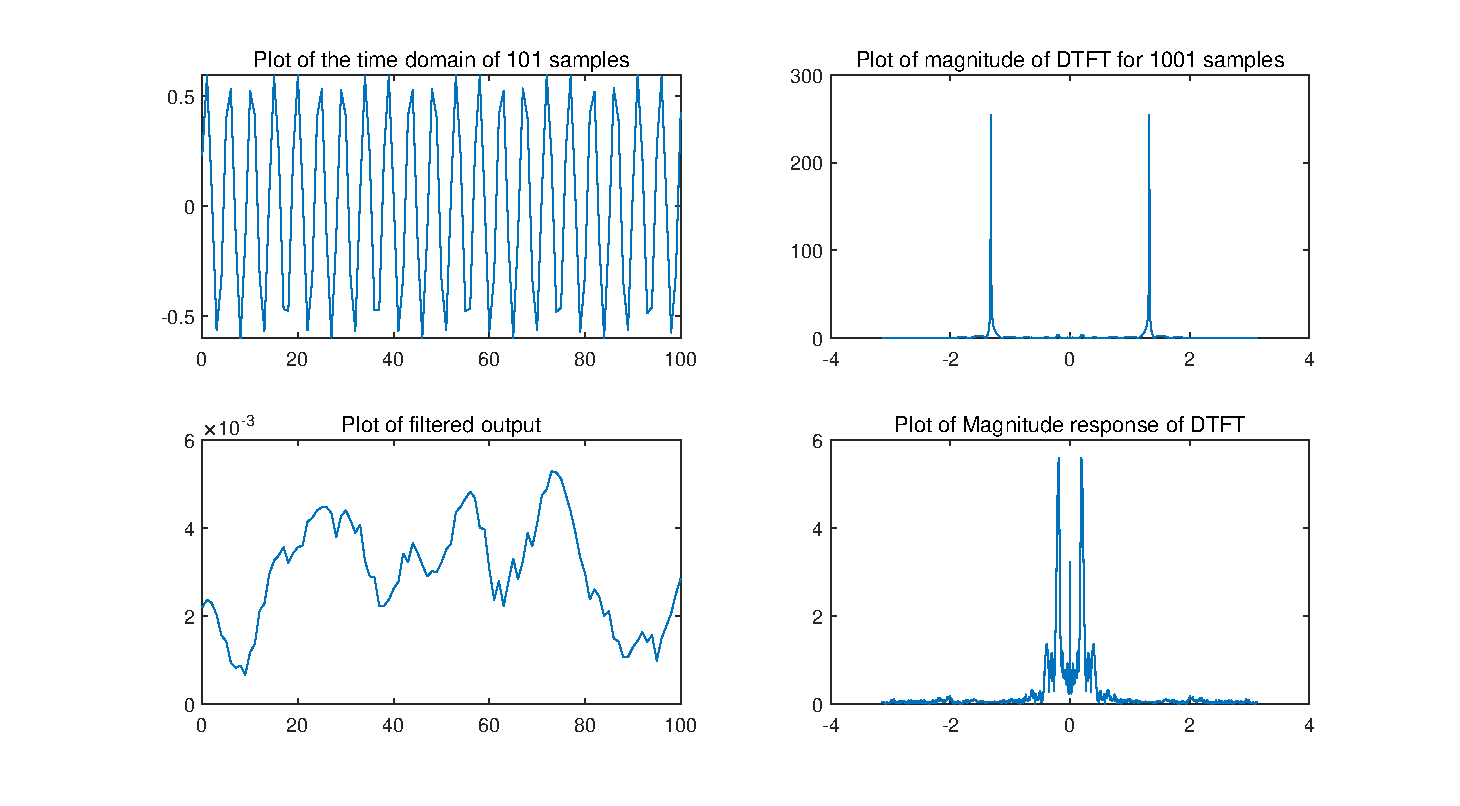
\includegraphics[width=170mm]{pictures/FIRfilter.eps}
		\caption{Effects of filtering.}
	\end{figure}
	\item Analysis:
	\begin{itemize}
		\item This is a bandpass filter.
		\item After filtering, the distance of impulses becomes lower in the frequency domain and the the waveform in the time domain changes a lot.
	\end{itemize}	
\end{itemize}
\section*{7.4 Design of a Simple IIR Filter}
\addcontentsline{toc}{section}{7.4 Design of a Simple IIR Filter}
\subsection*{Question 1:}
\begin{itemize}
	\item Analytical transfer function:
	$$
	H_i(z)=\frac{1-r}{1-2r\cos\theta z^{-1}+r^2z^{-2}}
	$$
	\item Difference equation:
	$$
	y[n]-2 r \cos \theta y[n-1]+r^{2} y[n-2]=(1-r) x[n]
	$$
	\item System diagram:
	\begin{figure}[H]
		\centering
		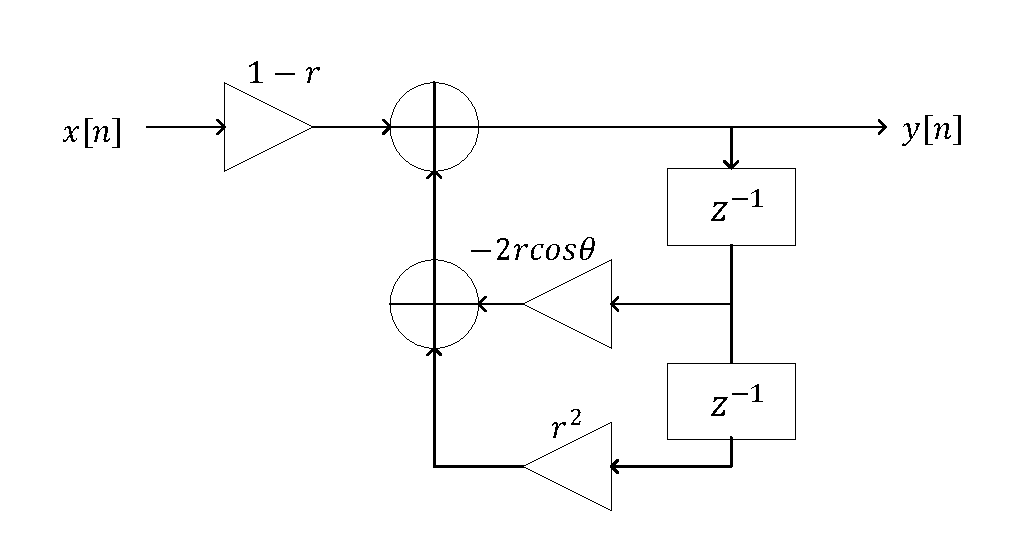
\includegraphics[height=70mm]{pictures/框图2.pdf}
		\caption{System diagram}
	\end{figure}
	\item q7\_4a.m:
\end{itemize}
\begin{lstlisting}[title=q7\_4a.m]
	clear;
	w=-pi:0.01:pi;
	z = exp(j*w);
	r1 = 0.99;r2 = 0.9; r3 = 0.7;
	Hi1 = (1-r1)./(1-2*r1*cos(pi/3).*z.^(-1)+(r1.^2)*(z.^(-2)));
	Hi2 = (1-r2)./(1-2*r2*cos(pi/3).*z.^(-1)+(r2.^2)*(z.^(-2)));
	Hi3 = (1-r3)./(1-2*r3*cos(pi/3).*z.^(-1)+(r3.^2)*(z.^(-2)));
	subplot(1,3,1);plot(w,abs(Hi1));title('r=0.99');
	subplot(1,3,2);plot(w,abs(Hi2));title('r=0.9');
	subplot(1,3,3);plot(w,abs(Hi3));title('r=0.7');	
\end{lstlisting}
\begin{itemize}
	\item Running result:
	\begin{figure}[H]
		\centering
		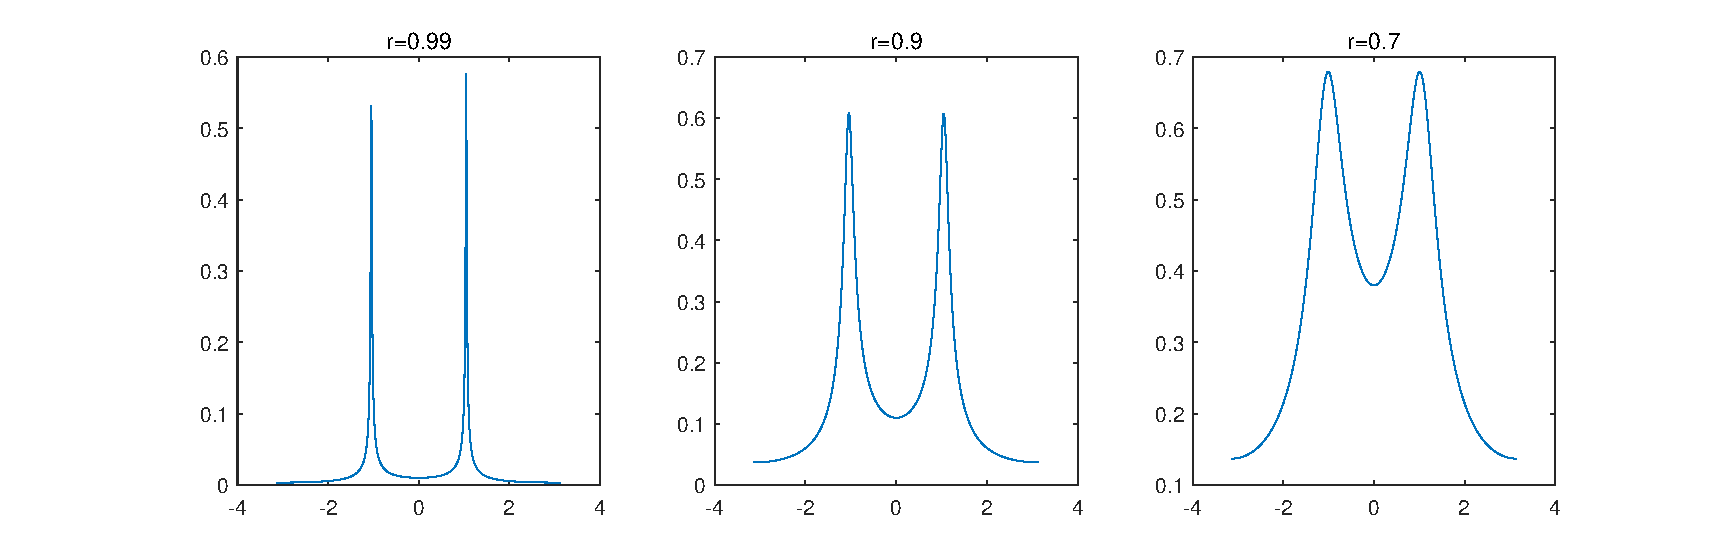
\includegraphics[width=170mm]{pictures/Hi.eps}
		\caption{$H_i$ with different $r$.}
	\end{figure}
	\item Analysis: As r decreases, the magnitude response would become smoother.
	(The width of two impulses would become larger. 
	And when $r \rightarrow 1$, the impulse could be considered as ideal impulse.)
\end{itemize}
\subsection*{Question 2:}
\begin{itemize}
	\item IIRfilter.m:
\end{itemize}
\begin{lstlisting}[title=IIRfilter.m]
	function y = IIRfilter(x)
	theta = (3146/8000)*2*pi;
	r = 0.995;
	N = length(x);
	y = zeros(1,N);
	y(1) = x(1);
	y(2) = x(2)+2*r*cos(theta);
	for i = 3:N
	y(i) = x(i)+2*r*cos(theta).*y(i-1)-(r^2).*y(i-2);
	end
	end
\end{lstlisting}
\begin{itemize}
	\item q7\_4b.m:
\end{itemize}
\begin{lstlisting}[title=q7\_4b.m]
	clear;
	load pcm;
	sig1 = pcm(100:200);
	sig2 = pcm(100:1100);
	n = 0:length(sig1)-1;
	[X,w] = DTFT(sig2,0);
	f = IIRfilter(pcm);
	f1 = f(100:200);
	f2 = f(100:1100);
	theta=(3146/8000)*2*pi;
	[F,w] = DTFT(f2,0);
	w1 = w(w>(theta-0.02));
	w1 = w1(w1<(theta+0.02));
	X1 = X(w>(theta-0.02) & w<(theta+0.02));
	f_X1 = F(w>(theta-0.02) & w<(theta+0.02));
	subplot(611),plot(n,sig1);title('101 samples of the orignal signal');
	subplot(612),plot(w,abs(X));title('magnitude of DTFT');xlim([-pi pi]);
	subplot(613),plot(n,f1);title('101 samples of the filtered output');
	subplot(614),plot(w,abs(F));title('magnitude of DTFT filtered output');xlim([-pi pi]);
	subplot(615),stem(w1,abs(X1));title('magnitude of DTFT in the range of the orignal signal');
	subplot(616),stem(w1,abs(f_X1));title('magnitude of DTFT in the range of the filtered output');
\end{lstlisting}
\begin{itemize}
	\item Running Result:
\end{itemize}
\begin{figure}[H]
	\centering
	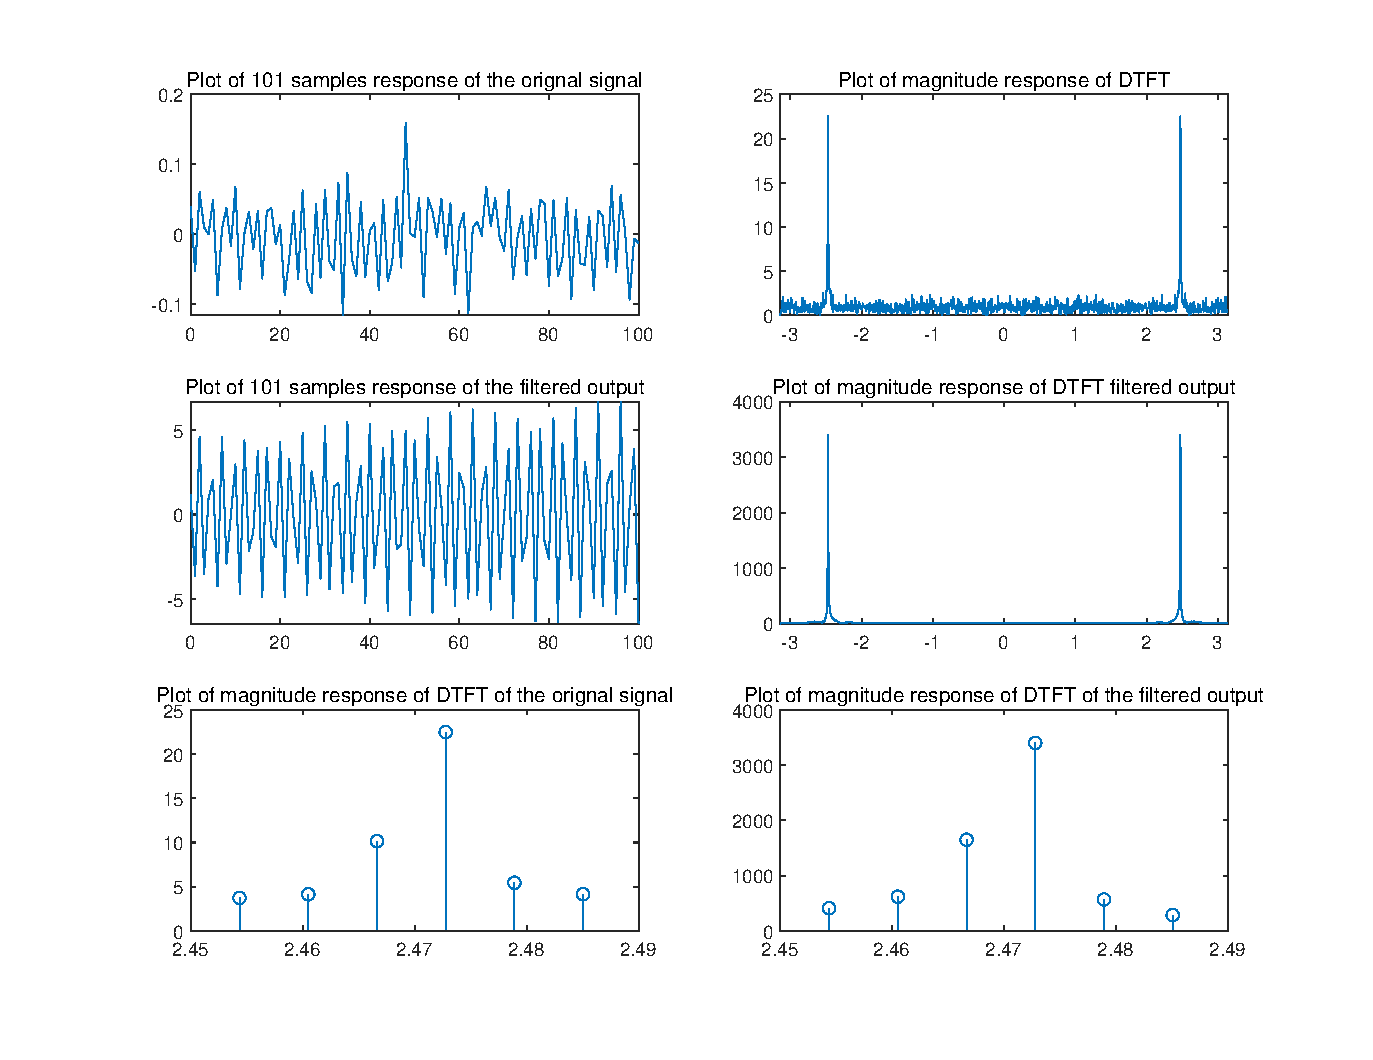
\includegraphics[width=170mm]{pictures/7.4b.eps}
	\caption{Six plots of Questions 2}
\end{figure}
\begin{itemize}
	\item Analysis: After filtering, the speech noise in the frequency domain decrease much more. Moreover, the sound after filtering is much more clearer.
\end{itemize}
\section*{7.6 Filter Design Using Truncation}
\addcontentsline{toc}{section}{7.6 Filter Design Using Truncation}
\begin{itemize}
	\item LPFtrunc.m and test codes:	
\end{itemize}
\begin{lstlisting}[title=LPFtrunc.m]
	function h=LPFtrunc(N)
	for i=1:N
	h(i)=2/pi*sinc(2/pi*(i-1-(N-1)/2));
	end
	end
\end{lstlisting}
\begin{lstlisting}[title=q7\_6.m]
	clear;
	load nspeech2.mat;
	N1=21;
	N2=101;
	h1 = LPFtrunc(N1);
	[X1,w1] = DTFT(h1,512);
	h2 = LPFtrunc(N2);
	[X2,w2] = DTFT(h2,512);
	figure(1);
	subplot(121),plot(w1,abs(X1));title("magnitude not in dB, N=21");
	subplot(122),plot(w2,abs(X2));title("magnitude not in dB, N=101");
	figure(2);
	subplot(121),plot(w1,20*log10(abs(X1)));title("magnitude in dB, N=21");
	subplot(122),plot(w2,20*log10(abs(X2)));title("magnitude in dB, N=101");
\end{lstlisting}
\begin{itemize}
	\item Running result:
	\begin{figure}[H]
		\centering
		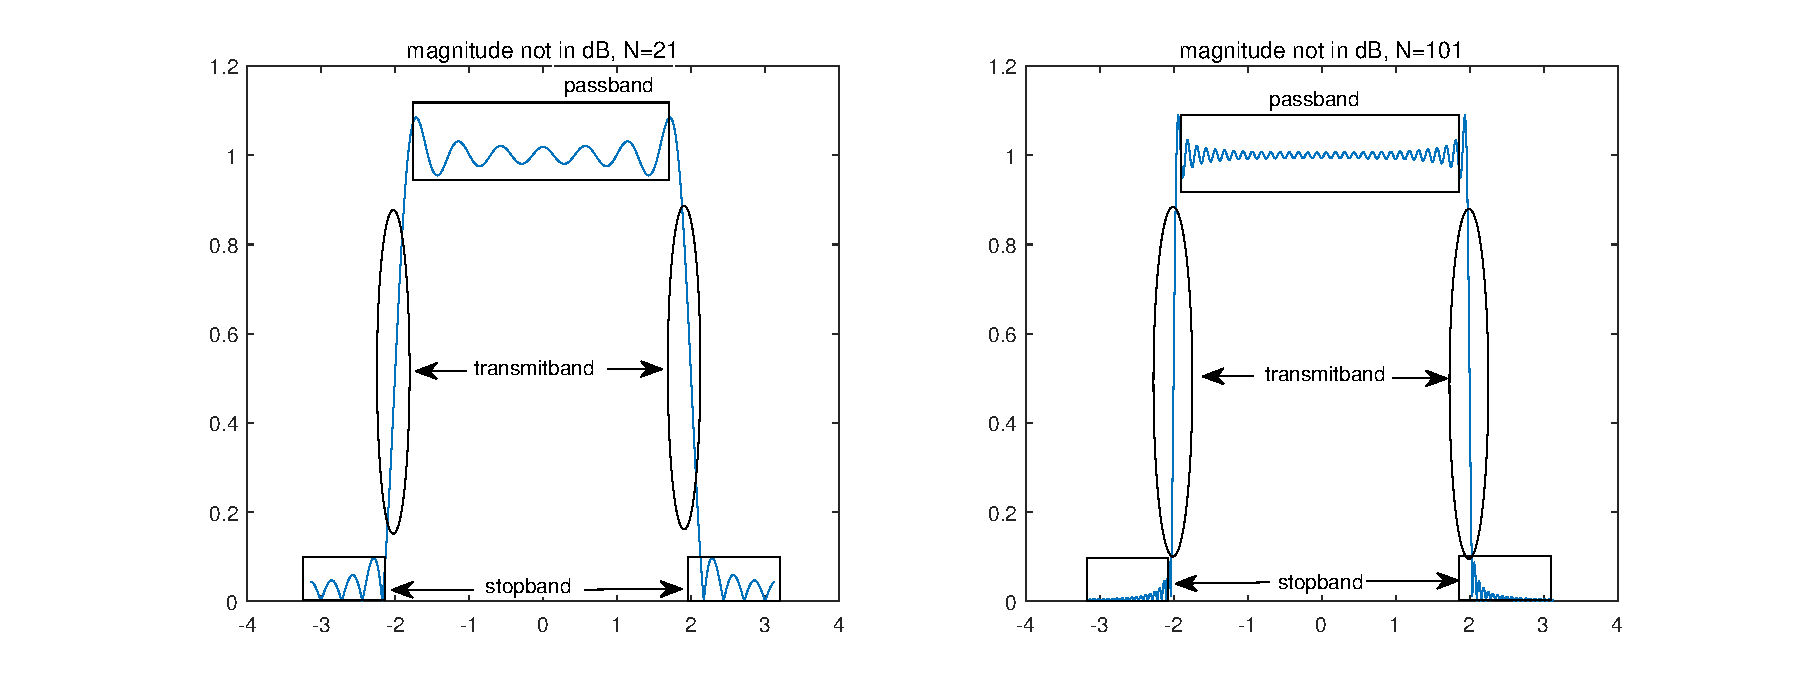
\includegraphics[width=170mm]{pictures/1.eps}
		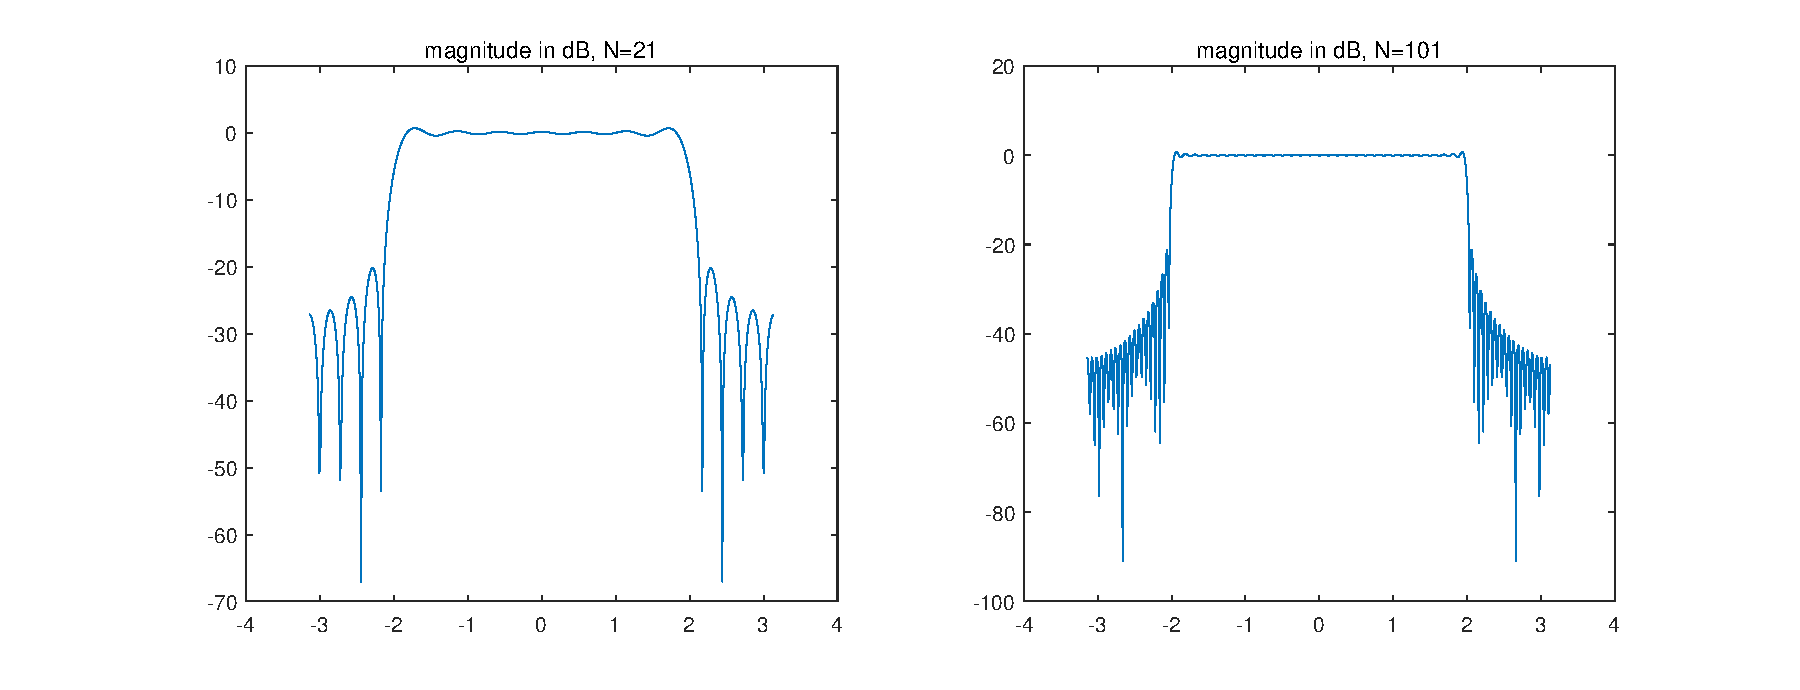
\includegraphics[width=170mm]{pictures/2.eps}
		\caption{Magnitude Response.}
	\end{figure}
	\item Analysis:
	\begin{enumerate}
		\item When N increases, the filtering becomes much more better because of the more sampling points.(Compare the Gibbs Phenomenon in the passband.)
		\item After filtering, the filtered result sounds much smoother, with fewer sharp tones.
	\end{enumerate}
\end{itemize}
\section*{8.2 Filter Design Using Standard Windows}
\addcontentsline{toc}{section}{8.2 Filter Design Using Standard Windows}
Running Result:
\begin{figure}[H]
	\centering
	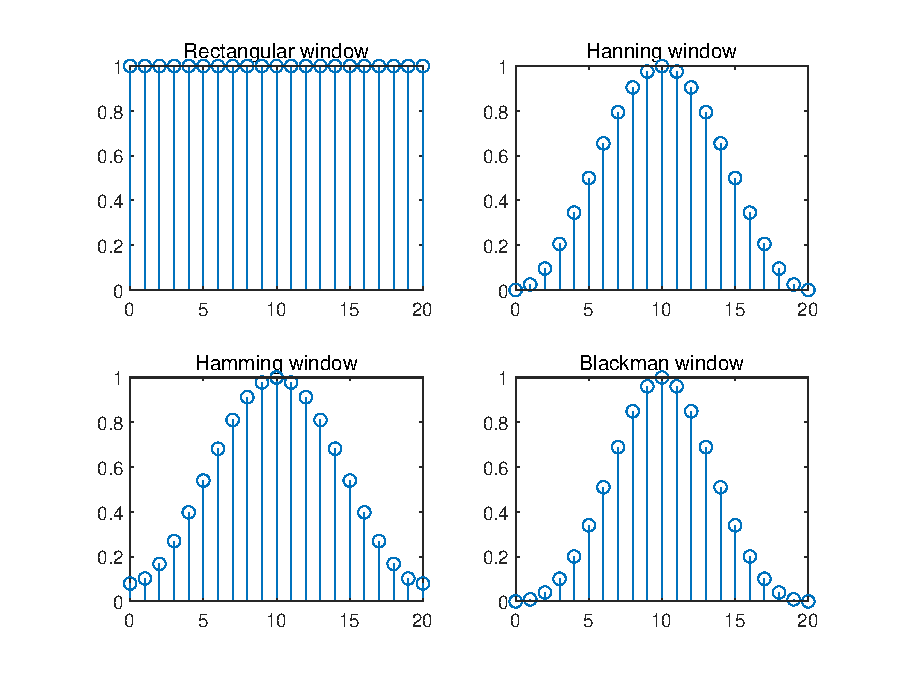
\includegraphics[width=150mm]{pictures/window1.eps}
	\caption{Time domain plots of the four windows.}
\end{figure}
\begin{figure}[H]
	\centering
	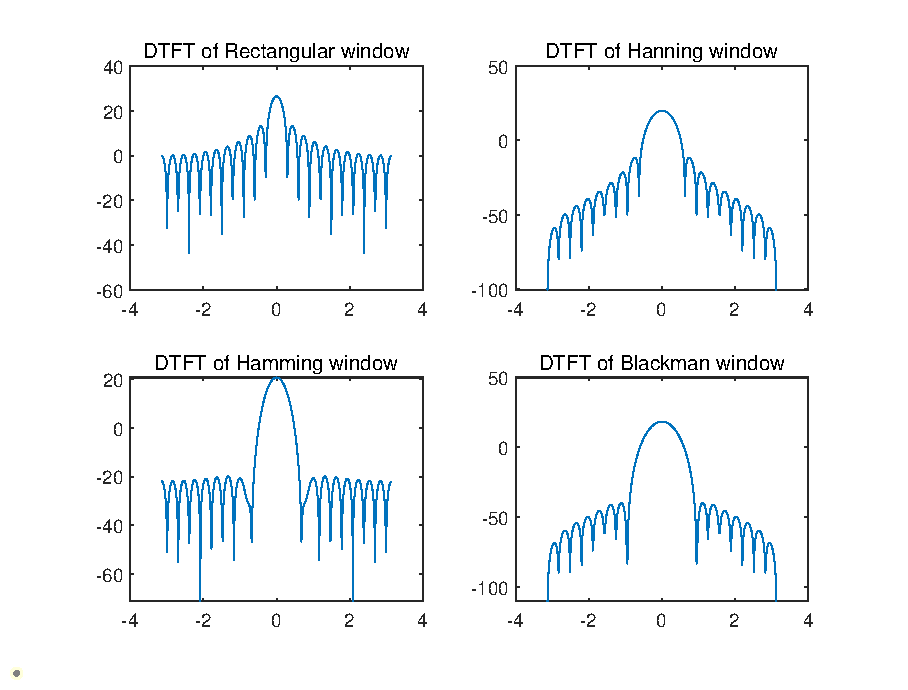
\includegraphics[width=150mm]{pictures/window2.eps}
	\caption{Frequency domain plots of the four windows.}
\end{figure}
\begin{figure}[H]
	\centering
	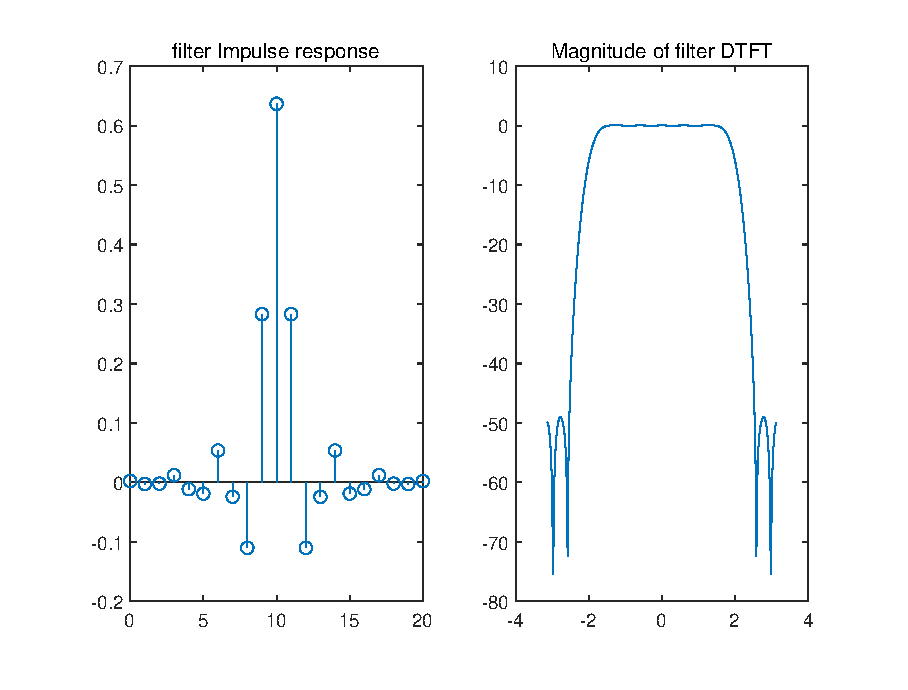
\includegraphics[width=150mm]{pictures/window3.eps}
	\caption{impulse response and magnitude of filter's DTFT}
\end{figure}
\begin{figure}[H]
	\centering
	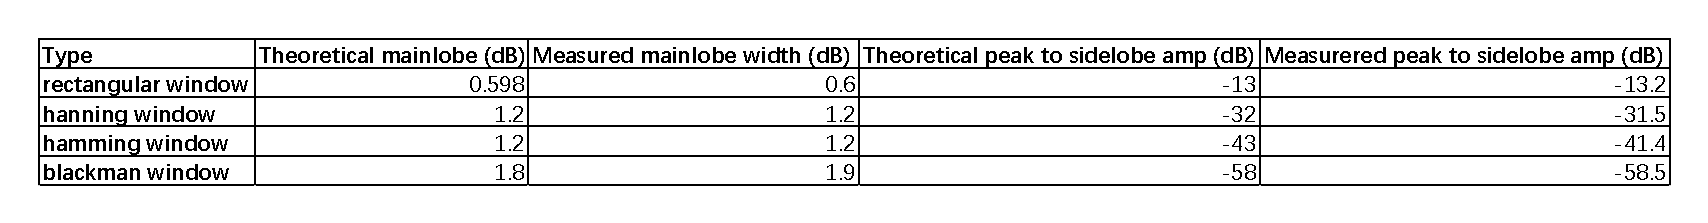
\includegraphics[width=180mm]{pictures/表格.pdf}
	Table of the measured and theoretical window spectrum parameters.
\end{figure}
Analysis:
\begin{enumerate}
	\item The theoretical result and measured result are very close.
	\item Performance comparison: blcak window > hamming window > hanning window > rectangular window.
	(Larger mainlobe widh and lower sidelobe.)
\end{enumerate}

\section*{8.3 Filter Design Using the Kaiser Window}
\addcontentsline{toc}{section}{8.3 Filter Design Using the Kaiser Window}
\newpage
\subsection*{Codes:}
\begin{lstlisting}[title=q8\_3.m]
	% For both Questions 1 and 2.
	clear;
	N=0:20;
	x1=kaiser(21,0);x2=kaiser(21,1);x3=kaiser(21,5);
	[X1,w1]=DTFT(x1,512);
	[X2,w2]=DTFT(x2,512);
	[X3,w3]=DTFT(x3,512);
	
	

	figure(1);
	sgtitle('three plots of Kaiser windows.');
	subplot(3,2,1);stem(N,x1);xlabel('n(s)');title('kaiser window for beta=0');
	subplot(3,2,2);plot(w1,20*log10(X1));xlabel('w(rad)');title('magnitude of DTFT for beta=0');
	subplot(3,2,3);stem(N,x2);xlabel('n(s)');title('kaiser window for beta=1');
	subplot(3,2,4);plot(w2,20*log10(X2));xlabel('w(rad)');title('magnitude of DTFT for beta=1');
	subplot(3,2,5);stem(N,x3);xlabel('n(s)');title('kaiser window for beta=5');
	subplot(3,2,6);plot(w3,20*log10(X3));xlabel('w(rad)');title('magnitude of DTFT for beta=5');
	
	

	figure(2);
	load nspeech2;
	beta=4.0909;N=51;
	w = kaiser(N, beta);
	h1 = LPFtrunc(N);
	h2 = h1.*w';
	[H,w] = DTFT(h2,512);
	sgtitle('three plots of magnitude response.')
	subplot(3,1,1);
	plot(w,20*log10(H));title('DTFT of filter in dB');
	subplot(3,1,2);
	plot(w(abs(w)<=1.8),20*log10(H(abs(w)<=1.8)));title('|w| <= 1.8 in dB');
	subplot(3,1,3);
	plot(w(abs(w)>=2.2),20*log10(H(abs(w)>=2.2)));title('|w| >= 2.2 in dB');
	f = conv(h2,nspeech2);
	[F,w] = DTFT(f,512);
	
	

	figure(3);
	plot(w,20*log10(F)); title('magnitude of filtered signal in dB');
	xlim([-3.5 3.5]);		
\end{lstlisting}
\newpage
\subsection*{Question 1:}
Running Result:
\begin{figure}[H]
	\centering
	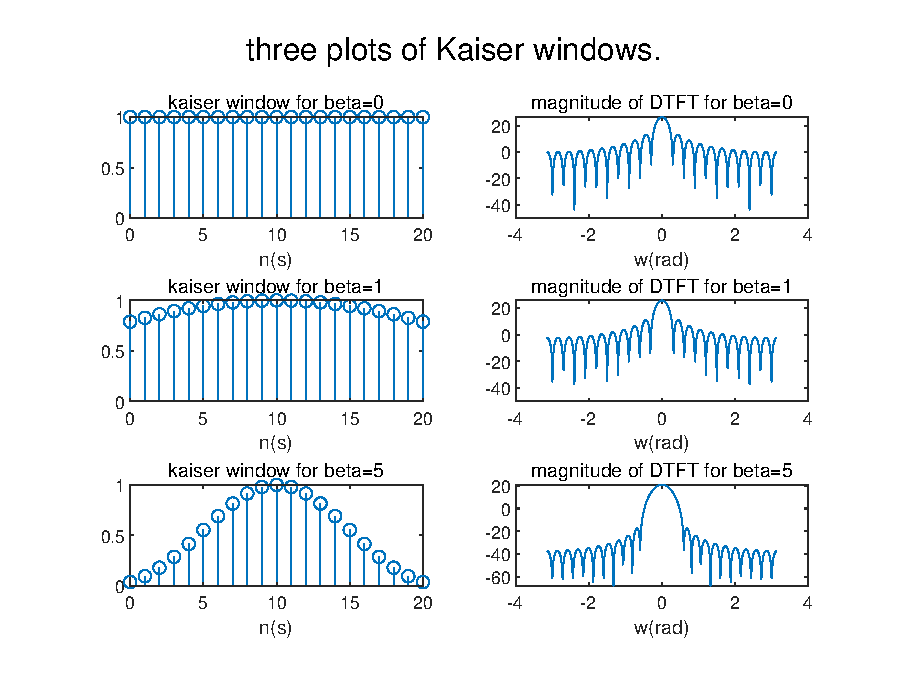
\includegraphics[width=170mm]{pictures/win1.eps}
	\caption{plots of the 3 Kaiser windows and the magnitude of their DTFT's indecibels.}
\end{figure}
Comment:\\
As $\beta$ increases, the time domian window becomes no more flat(Two sides of the window decrease.).
Moreover, in the frequency domian, sidelobes gradually decrease.
\subsection*{Question 2:}
Calculate $\beta$ and $N$:
$$
\omega[n]=\left\{\begin{array}{ll}I_{0}\left(\beta \frac{\sqrt{n(N-1-n)}}{N-1}\right) \\\frac{1}{I_{0}(\beta)} & n=0,1, \ldots, N-1 \\0 & \text { otherwise }\end{array}\right.
$$
$$
\beta=\left\{\begin{array}{lr}0.1102(A-8.7) & A>50 \\\left\{0.5842(A-21)^{0.4}+0.07886(A-21)\right. & 21 \leq A \leq 50 \\0.0 & A<21\end{array}\right.
$$
$$
N=\left[1+\frac{A-8}{2.285\left(\omega_{s}-\omega_{p}\right)}\right]
$$
$\therefore$ $\beta=4.0909, N=51$.
Running Result:
\begin{figure}[H]
	\centering
	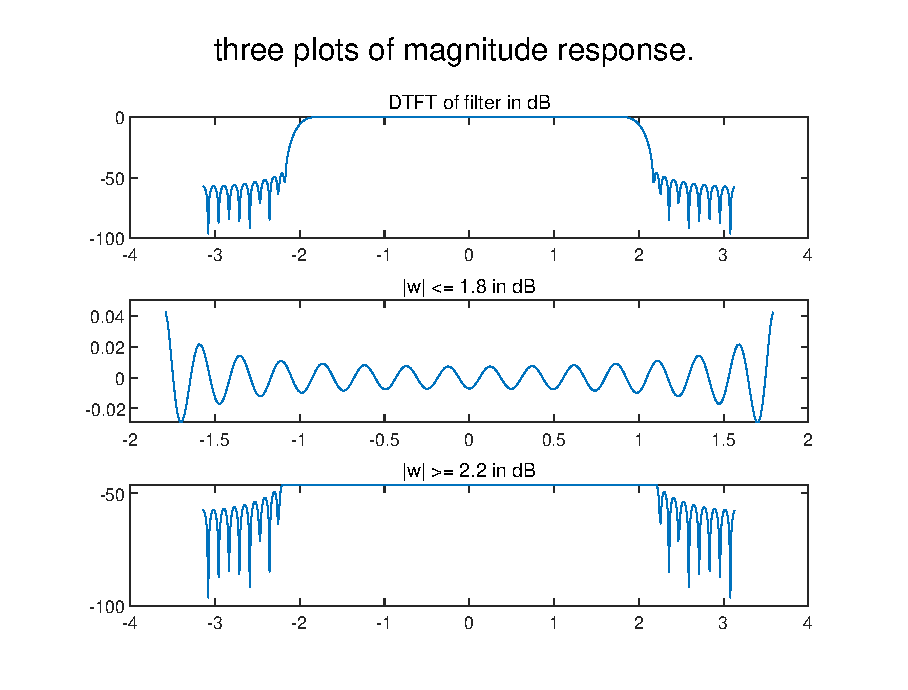
\includegraphics[width=150mm]{pictures/win2.eps}
	\caption{three plots of magnitude response.}
\end{figure}
\begin{figure}[H]
	\centering
	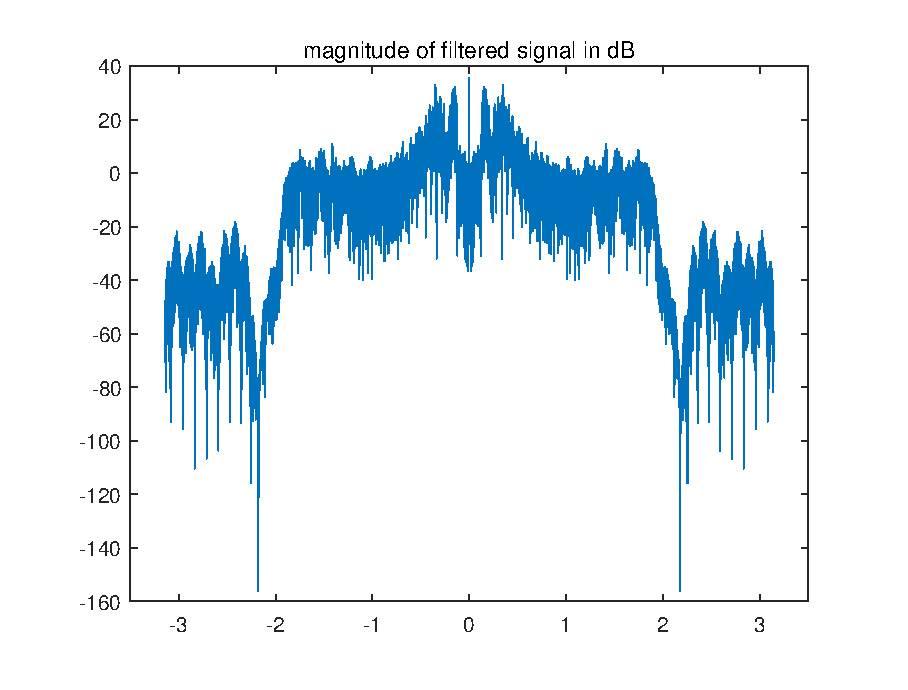
\includegraphics[width=150mm]{pictures/win3.eps}
	\caption{magnitude of filtered signal in dB}
\end{figure}
Analysis:
\begin{enumerate}
	\item After filtering, noise and sidelobe decrease. The DTFT becomes smoother.
	\item Filtered sounds are better and clearer.
\end{enumerate}
\section*{Summary}
\addcontentsline{toc}{section}{Summary}
\begin{info}
	这里拿中文写了$\ddot\smile$。 
\end{info}  
\begin{itemize}
	\item \textbf{关于这篇报告:}
	\\对于这个篇报告,我有一点小遗憾。其实最初原本想拿latex写一个像之前几次Lab一样较为完美的学术报告,但是由于各种期末考试的压力,我这篇报告在考试后才完成,因此显得有一些虎头蛇尾。
	但是总得来说,通过这次实验的各种小型实验,我对IIR和FIR滤波器的设计都有了一定程度的理解,也获得不了不少宝贵的编程经验以及分析问题的能力。显然这是更为重要的。
	\item \textbf{关于整个学期:}
	\begin{itemize}
		\item 	说实话,虽然这个学期学业比较繁重,但是我还是收获了不少东西:从MATLAB,Simulink的基本使用,再到对信号处理的一些函数的复现,以及后来深入的滤波器设计和计算机生成音乐的Mini Project,
		这都是我前所未有的经验,也让我感受到了作为一个“工程师”的快乐。
		\item 另外,对于每次LAB课报告的撰写,我也收获很多。譬如,为了科学严谨的叙述问题,我开始采用更多的数学语言描述问题或是使用visio绘制流程图。为了让自己的排版更加精美,我也逐渐尝试了从word,到markdown再到Latex的排版方法。
		同样的,我也逐渐熟悉了Latex公式的编写并设置自己的Latex模板。我认为,这些都是我自己这学期超越分数最为宝贵的经验,为自己将来的科研和学习打下坚实的基础。
	\end{itemize}
	\item \textcolor{red}{最后,感谢老师和学助对我们的指导和关心!}
\end{itemize}
\section*{Appendix}
\addcontentsline{toc}{section}{Appendix}
\begin{lstlisting}[title=DTFT.m]
	function [X,w] = DTFT(x,M)
	% This function computes samples of the DTFT of x. 
	% To compute the DTFT of x, use
	%
	%             [X,w] = DTFT(x,0)
	%
	% where X is the vector of DTFT samples and w is the 
	% vector of radial frequencies. To compute at least
	% M samples of the DTFT, you may use the command
	%
	%             [X,w] = DTFT(x,M)
	%
	% This is useful when the plot of X versus w does
	% not contain a sufficient number of points.
	N = max(M,length(x));
	N = 2^(ceil(log(N)/log(2)));
	% Take the padded fft
	X = fft(x,N);
	w = 2*pi*( (0:(N-1))/N );
	w = w - 2*pi*(w>=pi);
	% Shift FFT to go from -pi to pi
	X = fftshift(X);w = fftshift(w);	
\end{lstlisting}
\end{document}